% SVM parameter
\newcommand{\svmT}{\bm{\theta}}
\newcommand{\svmB}{b}
\newcommand{\svmAug}{\tilde{\svmT}}
%\newcommand{\svmAugAll}{\svmAug_{\text{all}}}
\newcommand{\svmAugAll}{\bm{\Theta}}

%\begin{figure}
%\begin{center}
%\subfigure[Early Adaptation]{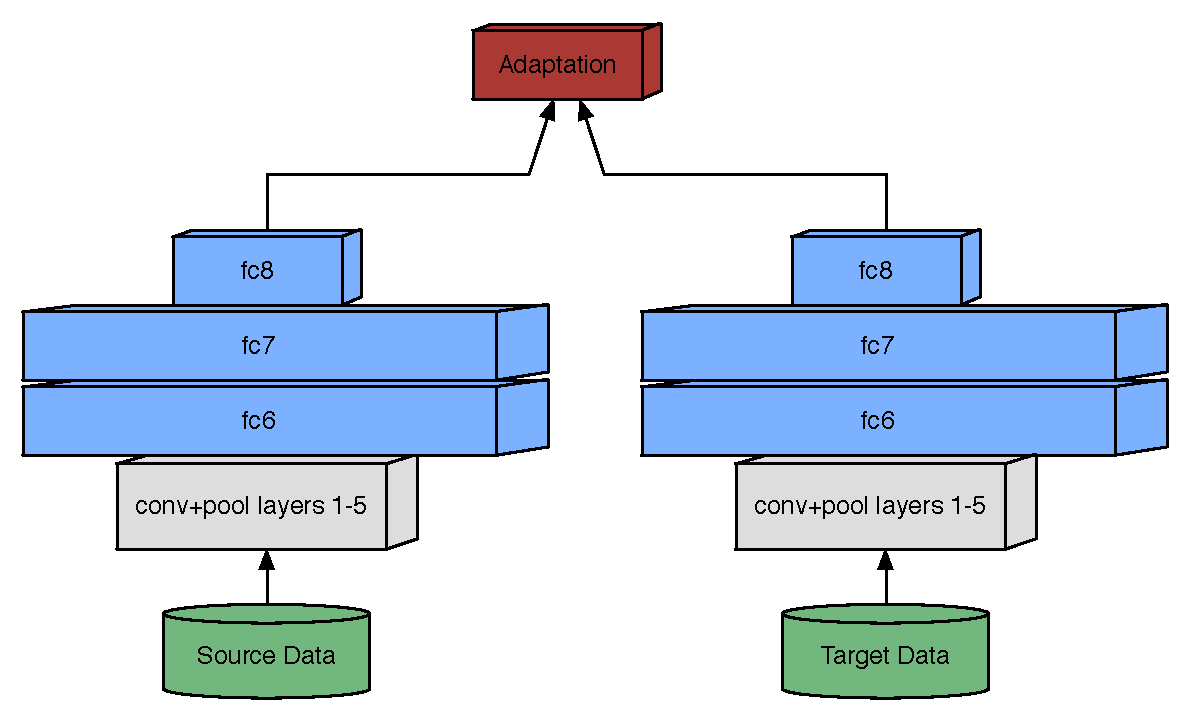
\includegraphics[width=.45\linewidth]{figs/model-adapt-unsuper}}
%\subfigure[Late Adaptation]{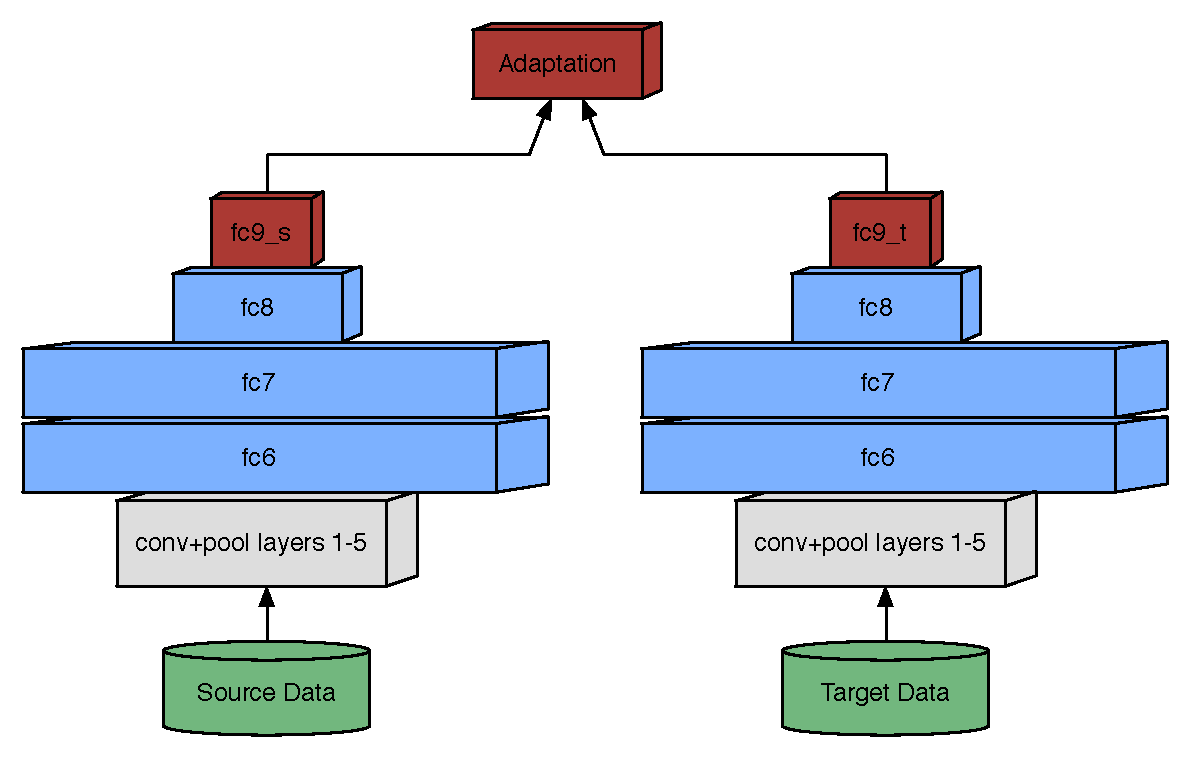
\includegraphics[width=.45\linewidth]{figs/model-adapt-super}}
%\end{center}
%\caption{Our proposed framework for adaptation. The source data and target data are each independently passed through the supervised convolutional neural network which has been trained on the 1.2Million images in the ILSVRC2012 Challenge dataset~\cite{ilsvrc2012}. We compute the subspace distance (A-distance) between the source and target data as it is represented in each of the fully connected layers of the network (represented in blue). The layer that produces the minimum subspace distance between source and target is chosen for adaptation. Finally, adaptation is performed on the activations from the best layer (shown in red).}
%\label{fig:model}
%\end{figure}

\begin{figure}
\begin{center}
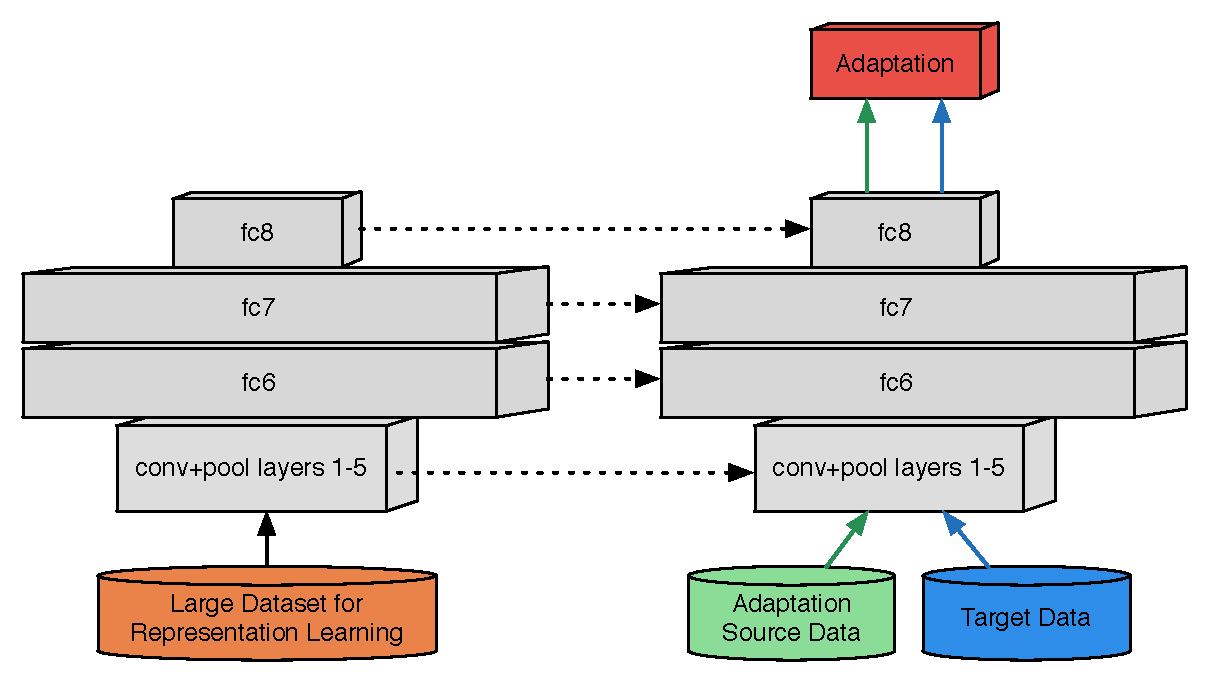
\includegraphics[width=.6\linewidth]{figs/model-adapt}
\end{center}
\caption{Our proposed framework for adaptation. We pre-train a supervised CNN using a large labeled source dataset (ImageNet). We then learn a model for use in the target domain by transferring the CNN parameters and training a new adaptation layer with source data and labeled (or unlabeled) target data.}
\label{fig:model-adapt}
\end{figure}

% Describe adaptation algorithms
%Many methods have been proposed for visual domain adaptation. 
% \ks{similar edit as in intro, see if this make sense}

We propose a general framework for selectively adapting the parameters of a
convolutional neural network (CNN) whose representation and classifier weights
are trained on a large-scale source domain, such as ImageNet. 
We begin by pre-training a supervised CNN using the architecture proposed by 
Krizhevsky et al~\cite{supervision}. This network has shown state of the art
performance for image classification and offers a strong starting model.

At test time, we assume we will receive data from the target domain. Therefore, we seek to 
learn to adapt the CNN so that it performs well on the target tasks. Unfortunately,
our CNN architecture contains millions of parameters and in many adaptation 
scenarios we have few or no labeled examples available at training time from the
target domain. Therefore, we suggest fixing the majority of the parameters in our 
network and learning a single adaptation layer that takes as input
the activations from the fixed network for the target training data as well as an auxiliary labeled
dataset which is available to us at adaptation time (source data). The source data
can, but doesn't have to be, the same data that was used to pre-train the network.

Figure~\ref{fig:model-adapt} illustrates our proposed framework for adapting a deep CNN 
with limited target data. We depict the transfer of all pre-trained layers to the final adapted model 
for simplicity of presentation,  however, in general, there is no reason to assume a priori that 
adding the adaptation layer after all pre-trained layers is the best approach.  Instead, we choose
the number of layers to transfer as a function of the source and target data.

Intuitively, when selecting a layer to use for adaptation, we would like to use
the one in which the source and target appear the most similar (and thus
experience the least domain shift).
To get at this notion of similarity, we make use of the concept of an A-distance
\cite{adist}. A-distance is a measure of distance between two subspaces and hence 
can be used to measure the distinguishability of two datasets.

We compute the A-distance metric on the source and target activations after each fully 
connected layer 
and automatically select the  layer after which
our source and target datasets are most similar, and hence most amenable to adaptation.

Given two domains $X_1$ and $X_2$, the A-distance between them is defined as:

\begin{equation}
  d_A(X_1, X_2) = 2 \left( 1 - 2 \min_{h' \in H} E(h'(X_1, X_2))\right)
\end{equation}


where $E(h^*(X_1, X_2))$ is the test error of the optimal hyperplane that attempts to
distinguish between the two domains.

In practice, it's NP-hard to find the optimal hyperplane, so we use a computationally simple and 
close approximation to the A-distance metric which was introduced by Ben-David et al~\cite{adist-comp}, 
where the optimal hyperplane is replaced by the classifier model parameter learned from a linear SVM.

Once we have selected which layer to use, we then add an adaptation layer to
the top of the architecture, as indicated in Figure~\ref{fig:model-adapt}. This layer
consists of an adaptation technique which combines the source and target
training data, then learns a linear classifier. In this paper, we look to the
standard domain adaptation literature and experiment using a variety of those
techniques. The key being that we need to use approaches that can operate with little or no
target training data.

%We are interested in both unsupervised and supervised settings, so we examine
%two sets of adaptation techniques. For the unsupervised setting, we use the
%Geodesic Flow Kernel (GFK)~\cite{gong-cvpr12} and Subspace Alignment
%(SA)~\cite{sa} methods. For the supervised setting, we use the Late Fusion,
%\daume~\cite{daume}, Projective Model Transfer (PMT)~\cite{aytar-iccv11}, and
%Max-margin Domain Transforms (MMDT)~\cite{hoffman-iclr13} methods.
